\chapter[Dataset and Simulation][Dataset and Simulation]{Dataset and Simulation}
\label{chapter:data} 

\section{Data}

\subsection{The 2012 Dataset} 

The \tth\ analysis uses the entire 2012 ATLAS dataset only, collected
from April to December. The size of the dataset corresponds to 20.3 \ifb, after passing data quality
requirements, ensuring the proper operation of the tracking, calorimeter and muon subsystems.  
The LHC successfully produced datasets for physics studies in 2010, 2011 and 2012. The 2012 
proton-proton dataset was delivered with collisions with a CME of 8 TeV with bunch collisions
every 50 ns\cite{Aad:2013ucp}.

Figure~\ref{figure:data_lumi} shows the accumulation of the 2012 dataset over time. 
Despite doubling the bunch spacing above the design of 25 ns, the luminosity neared
the design luminosity due to unexpected improvements in the transverse beam profile\cite{Carli:1424362}. This increased
the amount of pile-up, or number of collisions per bunch crossing and in general collision
events were busier due to these multiple interactions. Figure \ref{figure:data_pileup} shows
the average number of interaction per bunch crossing for the 2011 and 2012 datasets. The 2012
dataset shows an average of 20-25 interactions. 

\begin{figure}[!t]
\centering 
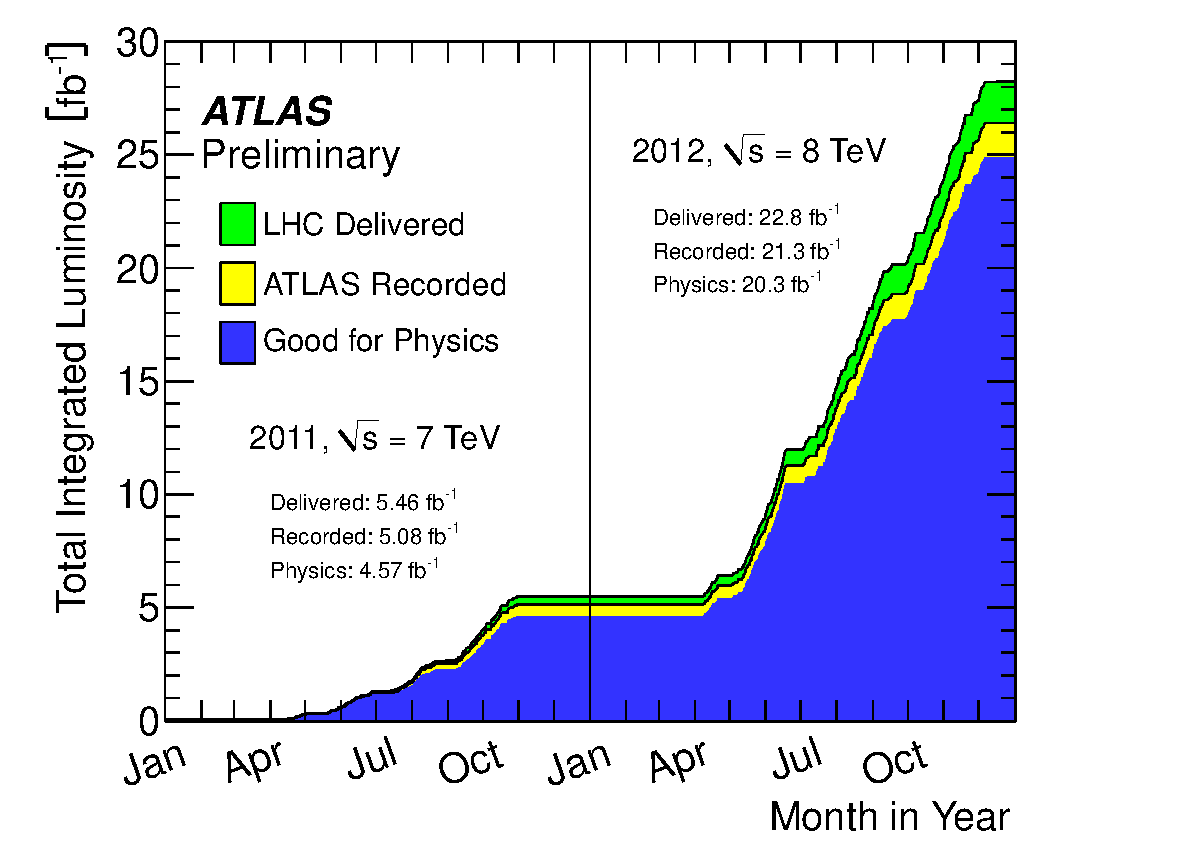
\includegraphics[width=0.60\textwidth]{figs/data/intlumivstime2011-2012DQ.pdf}
\caption{ Plot showing the accumulation of the integrated luminosity delivered to the ATLAS experiment over 2011 and 2012. The rough size of the usable, physics ready dataset for 2012 is 20 \ifb and is the dataset used. 
}
\label{figure:data_lumi}
\end{figure}


\begin{figure}[!t]
\centering 
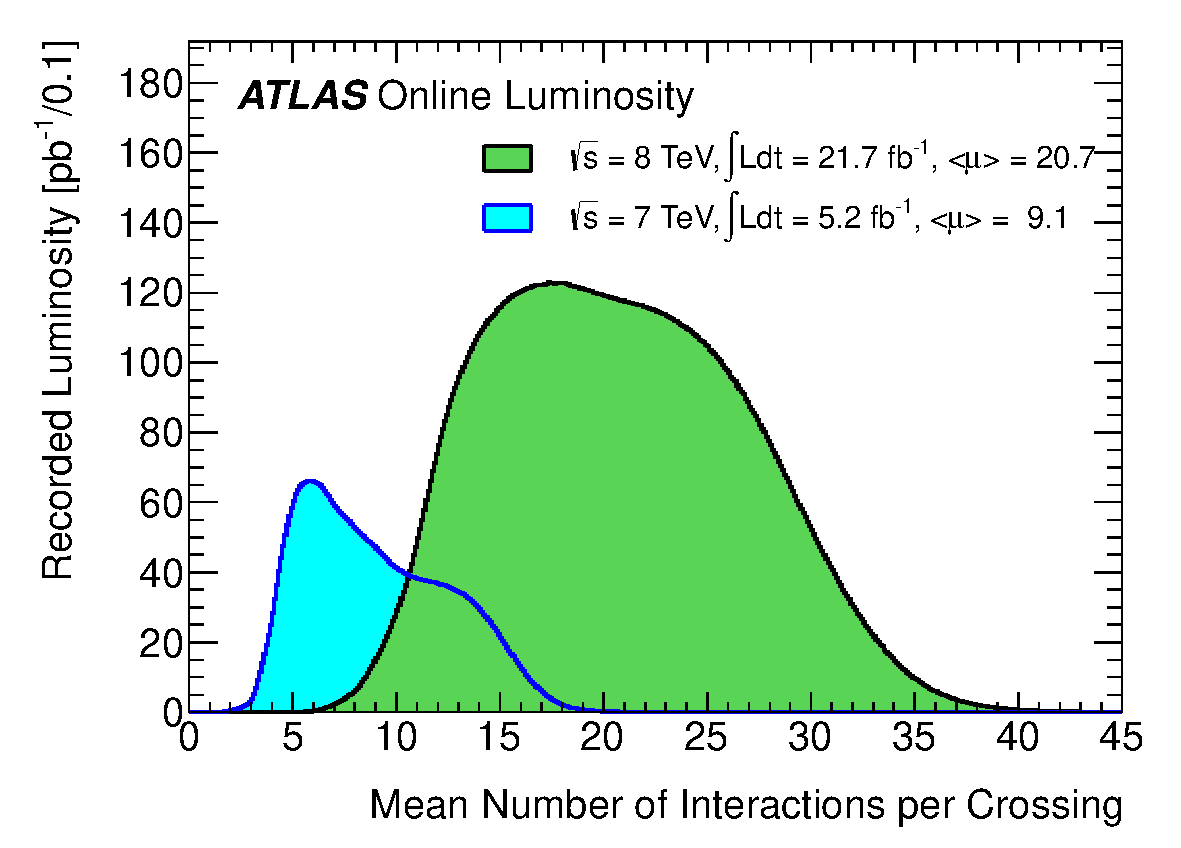
\includegraphics[width=0.60\textwidth]{figs/data/mu_2011_2012-dec.pdf}
\caption{ The average number of interactions per bunch-crossing for the 2012 and 2011 LHC proton-proton dataset. Most of these interactions are uninteresting but leave energetic signatures in particle detectors called pile-up which interfere with measurements}\label{figure:data_pileup}
\end{figure} 

The dataset must contain either a primary muon or primary electron trigger 
(\texttt{EF\_e24vhi\_medium1} OR \texttt{EF\_e60\_medium1} OR \texttt{EF\_24i\_tight} OR \texttt{EF\_36\_tight}). 
The electron triggers require a electron
with at least 25 \gev\ of calorimeter energy, passing the medium identification
requirement and loose tracking isolation.  Above 60\gev, the isolation
requirement is dropped and the identification is loosened slightly. 
The muon trigger requires a good inner detector track and matching
hits in the muon spectrometer, as well as loose tracking isolation,
which is also dropped about 36 GeV.  
            
\section{Simulation}

Simulation samples are used to determine the 
overall event selection acceptance and efficiency and model the number of events in the signal regions
for prompt backgrounds and signal. The simulated samples are created using parton distribution function (PDF) and
use Monte Carlo (MC) techniques to model the hard parton scatter, underlying event activity and parton showering and hadronization. 
The samples are then passed through a full ATLAS detector simulation\cite{Aad:2010ah} based on \textsc{GEANT4} \cite{Agostinelli:2002hh}.
Small corrections are then applied to re-scale object identification efficiencies,
energy scales, and the pile-up based on control regions from data. These corrections are discussed in Chapter~\ref{chapter:systematics}. 

\subsection{Signal Simulation}


The \ttbar$H$ production is modeled using matrix elements obtained from the HELAC-Oneloop package~\cite{Helac} that corresponds to the next-to-leading order (NLO) QCD accuracy. Powheg BOX~\cite{powheg,powbox1,powbox2} serves as an interface to the parton shower Monte Carlo programs. The samples created using this approach are referred to as {\textsc PowHel} samples. {\textsc CT10NLO} PDF sets are used and the factorization ($\mu_{\rm F}$) and renormalization ($\mu_{\rm R}$) scales are set to $\mu_{0} = \mu_{\rm F} = \mu_{\rm R} = m_{t}+\mH/2$. Pile-up and the underlying events are simulated by {\textsc Pythia} 8.1~\cite{PythiaManual8} with the {\textsc CTEQ61L} set of parton distribution functions and AU2 underlying event tune. The Higgs boson mass is set to $125\gev$ and the top quark mass is set to $172.5\gev$.\\
The signal Monte Carlo samples are summarized in Table~\ref{table:data_mcsignal}.
These large samples are generated with inclusive Higgs boson decays with
branching fractions set to the LHC Higgs Cross Section Working Group (Yellow Report)
recommendation for $m_H = 125$ GeV \cite{Heinemeyer:2013tqa}. The inclusive cross section (129.3
fb at $m_H = 125$ GeV) is also obtained from the Yellow Report \cite{Heinemeyer:2013tqa}.


\begin{table}
\begin{center} 
    \caption{Monte Carlo samples used for signal description.}\label{table:data_mcsignal}
   \begin{tabular}{l|c|c|c|c} 

      \hline\hline
       Process & Generator & Cross- & $\mathcal{L}$ [\ifb]  & Detector \\ 
               &           & section [fb] &            &  simulation \\
\hline
 ttH$\rightarrow$allhad+H & PowHel+Pythia8 & 59.09 & 2146.5 & Full \\
 ttH$\rightarrow$ljets+H & PowHel+Pythia8 & 56.63 & 2238.9 & Full \\
 ttH$\rightarrow$ll+H & PowHel+Pythia8 & 13.58 & 9332.0 & Full \\
\hline\hline
    \end{tabular}
  \end{center}
\end{table}


\subsection{Background Simulation}

The background simulations used for this analysis are listed in
Table~\ref{table:data_MCbackground}.  In general, the Alpgen\cite{Mangano:2002ea}, MadGraph\cite{Maltoni:2002qb}, and AcerMC\cite{Kersevan:2004yg} samples use the CTEQ6L1\cite{Nadolsky:2008zw}
parton distribution function, while the Powheg\cite{Frixione:2007vw}, Sherpa\cite{Gleisberg:2008ta}, are generated with the CT10 PDF.  The exception is the MadGraph $t\bar t t \bar t$ sample, which is generated with the
MSTW2008 PDF\cite{Martin:2009iq}. The highest order calculations available are used for the cross sections.  


\begin{table}
\begin{center} 
    \caption{Monte Carlo samples used for background
      description.  Unless otherwise specified MadGraph samples use Pythia 6
      for showering and Alpgen samples use Herwig+Jimmy. \ttbar, single top, and \zj~ samples are replaced with data-driven estimates for the final result}\label{table:data_MCbackground}

\begin{tabular}{l|l|c}
      \hline\hline
       Process & Generator   & Detector \\ 
               &             &  simulation \\
      \hline\hline
\ttW,\ttZ & MadGraph & Full \\
\tZ       & MadGraph & AF2 \\
$t\bar t t \bar t$ & MadGraph & Full \\
\ttWW & Madgraph+Pythia8  & AF2 \\
\ttbar & Powheg+Pythia6  & Full/AF2 \\
single top tchan & AcerMC+Pythia6& Full \\
single top schan$\rightarrow$l   & Powheg+Pythia6 & Full \\
single top $W^{\pm}t$ & Powheg+Pythia6 & Full \\
W$\gamma$*& MadGraph & Full \\
W$\gamma$+4p & Alpgen & Full \\
\WW & Sherpa &  Full \\
\WZ & Sherpa &  Full \\
Same-sign WW & Madgraph+Pythia8 & AF2 \\
ZZ& Powheg+Pythia8,gg2ZZ+Herwig & Full \\
Z$\gamma$*  & Sherpa  & Full \\
Z+jets & Sherpa & Full \\
ggF Higgs & Powheg+Pythia8 & Full \\
\end{tabular}
\end{center}
\end{table}


